\documentclass[12pt,onecolumn,a4paper]{article}
\usepackage{epsfig,graphicx,subfigure,amsthm,amsmath}
\usepackage{color,xcolor}     
\usepackage{xepersian}
\settextfont[Scale=1.5]{BZAR.TTF}
\setlatintextfont[Scale=1]{times-new-roman.ttf}
\graphicspath{{/sources}}





\begin{document}
\title{یک روش جدید برای پردازش کلان داده}
\author{احسان کریمی و علی صدقی \\
دانشگاه شهید بهشتی \\ درس آزمایشگاه پایگاه داده}
\date{\today}
\maketitle

\section{مقدمه}
نرم‌افزارهای یادگیری ماشین، چه به‌صورت بانظارت، چه به‌صورت بی‌نظارت، دردنیای واقعی بسیار کاربرد دارند. با توجه به دامنه و اندازه داده‌ها، امروزه مشکلات کلان‌داده بسیار معروف هستند.
مشکلات کلان‌داده، سه ویژگی مهم دارند. \\
حجم: همانطور که از اسم کلان‌داده مشخص است، حجم داده‌ها در آن بسیار زیاد است، و از گیگابایت، به ترابایت، و حتی پتابایت می‌رسد. با افزایش حجم داده‌ها، امکان ذخیره‌سازی داده برروی یک ماشین وجود ندارد.
و باید از چند ماشین برای این‌کار استفاده شود. با افزایش تعداد ماشین‌ها احتمال دردسترس نبودن آن‌ها بیشتر می‌شود، پس باید هرداده برروی چند ماشین ذخیره شود. به این‌کار \lr{replication} گفته می‌شود.
و یک کانفیگ محبوب برای این‌کار، مشخص کردن عدد ۳ برای آن است. در این‌حالت، هر داده، برروی سه ماشین ذخیره می‌شود. و با ازبین رفتن حداقل سه ماشین، قطعا ازدست دادن داده خواهیم داشت.
اما با از دست دادن یک یا دو ماشین، هیچ مشکلی برای ما به‌وجود نخواهد آمد. \\
سرعت: سرعت رسیدن داده به برنامه بسیار زیاد است. این مقدار از هزار، فراتر رفته و به میلیون رکورد در ثانیه هم می‌رسد. \\
تنوع: با بالارفتن حجم داده، تنوع آن نیز زیاد خواهد شد. به‌طور کلی داده‌ها به سه‌دسته‌ی ساختاریافته، نیمه‌ساخت‌یافته، و بی‌ساختار تقسیم می‌شود.
برای مثال در صفحات وب موجود در اینترنت، صفحاتی قسمت‌هایی دارند،‌که بقیه صفحات آن‌را ندارند. برای مثال صفحه‌ای بخش نظرات، دارد. برای ذخیره‌سازی صفحات وب، و با وجود این مشکل، دیگر نمی‌توانیم از \lr{RDBMS}ها استفاده کنیم.
داده‌های ساختاریافته، داده‌های موجود در \lr{RDBMS}ها هستند، که دقیقا مشخص است، هر رکورد چه ویژگی‌ها و رفتارهایی دارد. با بالارفتن حجم ، ممکن است، ویژگی‌های دو رکورد از یک نوع با یکدیگر برابر نباشد.
چون با افزودن این ویژگی برای تمام رکوردها، مقدار آن برای بسیاری از رکوردها، خالی، خواهد بود. اصطلاحا به این نوع جداول، \lr{sparce} گفته می‌شود. \\
به این سه ویژگی \lr{vvv} گفته می‌شود. چون معادل حجم، سرعت، و تنوع، در زیان انگلیسی، \lr{volume}، \lr{velocity}، و \lr{variety} می‌باشد.\\

\subsection{نیاز به تحلیل کلان‌داده}
در کلان‌داده، داده، با جزییات فراوان وجود دارد، پس پردازش داده در یک محیط توزیع‌شده، می‌تواند، همراه با خطای بسیار زیاد باشد. برای مثال اگر یک فیل وجود داشته باشد،
و چند انسان نابینا، با توجه به حس لامسه خود بخواهند، حدس بزنند، که این چه چیزی است، فردی با لمس پای فیل، تصور می‌کند، که یک درخت است.
فردی با لمس بدن فیل،‌ تصور می‌کند، دیوار است. فردی با لمس خرطوم آن، تصور می‌کند مار است. \\
همین مشکل، برای ماشین‌های مختلف وجود دارد. اگر هر قسمت از داده، در یک ماشین قرار گیرد، هر ماشین ممکن است،‌ تصور اشتباهی نسبت به داده، داشته باشد. برای حل این مشکل،
باید داده‌ها در یک قسمت تجمیع،‌ شود، و برروی آن تحلیل انجام شود. \\

\begin{figure}[h!]
\centering
	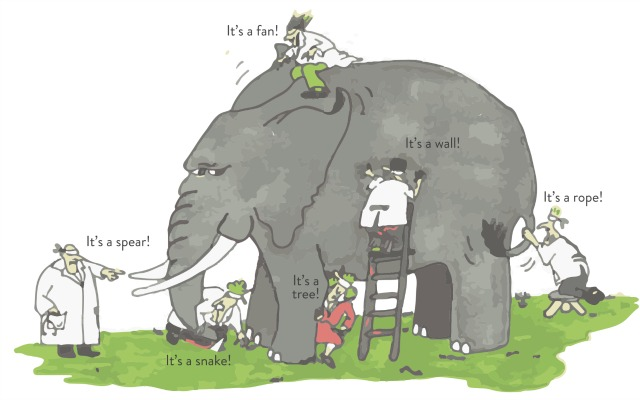
\includegraphics[width=1.2\textwidth]{elephant-and-blinds.jpg}
	\caption{ نگاه محدود و بایاس شده}
\end{figure}

\subsection{تکامل کلان‌داده}
آغاز تکامل کلان‌داده، از سال ۱۹۶۸ بود. اما این امر طی یک یا دو سال محقق نشد. بلکه در دوره‌های زمانی، پیوسته پیشرفت داشت. در ۱۹۶۸ پردازش تراکنش برخط یا \lr{OLTP}، با ظهور تراکنش‌های روزانه در پایگاه‌داده به‌وجود آمد.
در ۱۹۸۳، تکنولوژی انبار داده ظهور پیدا کرد. که این امر به دستاوری به داده‌های تاریخی کمک کرده‌است، که از \lr{OLTP} برای داده‌کاوی استفاده می‌شود.

\subsection{برنامه‌نویسی نگاشت-کاهش}
برنامه‌نویسی نگاشت-کاهش، یک رویکرد جدید برپایه‌ی برنامه‌نویسی شی‌گرا است، که معمولا با زبان جاوا پیاده‌سازی می‌شود. همانطور که از اسم آن پیداست، برنامه به دو قسمت نگاشت و کاهش، تقسیم می‌شود.
همانطور که قبلا اشاره کردیم، هر فایل به چند قسمت تقسیم می‌شود، و هر قسمت برروی یک ماشین، ذخیره می‌شود. در قسمت نگاشت، برنامه برروی تمام ماشین‌های صاحب داده یا \lr{datanode}ها اجرا می‌شود. و داده‌ی برروی ماشین‌را،
به مجموعه‌ای از کلیدها و مقدارها نگاشت می‌کند. برای مثال تمام کلمات موجود در آن بخش فایل‌را در اختیار می‌گیرد، و هرکدام از کلمات‌را به یک کلید و مقدار نگاشت می‌کند، که کلید آن، همان کلمه، و مقدار آن، برابر ۱ است. \\
حال در قسمت کاهش، هرکلید، با تمام مقادیر مقابل آن در اختیار برنامه خواهند بود. و خروجی یک مجموعه از کلیدها و مقدارها است. برای مثال، خروجی نگاشت مرحله‌ی قبل، که شامل کلمه و عدد بود، به صورت کلمه، و لیستی از اعداد، به برنامه داده می‌شود.
حال برنامه با جمع‌کردن، این مقادیر می‌تواند تعداد تکرار آن کلمه، در فایل‌را به‌دست آورد. \\
این رویکرد یک اشکال دارد. و آن این‌است، که در صورتیکه تعداد کلمات زیاد شود، به تعداد تکرار هر کلمه، کلید و مقدار خروجی در مرحله نگاشت، باید از طریق شبکه، به یک ماشین برسد. پس استفاده از شبکه در آن زیاد می‌شود.
پس بهتر است، قبل از ارسال خروجی، به ماشین مقصد، یکبار اعمال کاهش برروی خروجی، اعمال شود، تا استفاده از شبکه بهینه شود. به این کار ترکیب گفته می‌شود.

\begin{figure}[h!]
\centering
        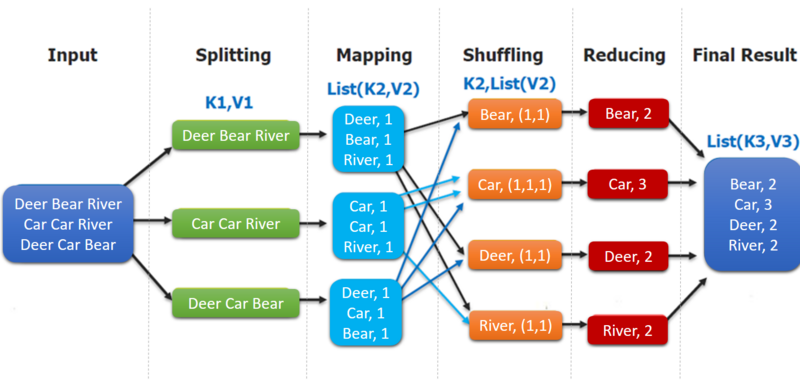
\includegraphics[width=1.0\textwidth]{hadoop-mapreduce.png}
        \caption{مراحل نگاشت کاهش در فریمورک هدوپ}
\end{figure}

\section{کارهای مرتبط}
یادگیری ماشین، افزودن هوش به برنامه است، تا برنامه بتواند یادبگیرد. پروسه‌ی یادگیری به دودسته‌ی یادگیری بانظارت، و بی‌نظارت تقسیم می‌شود. انواع روش‌های یادگیری ماشین در موارد شماره ۱ تا ۶ در منابع یافت می‌شوند.
این تکنیک‌ها در دنیای واقعی نیز مورد استفاده قرار می‌گیرند. \\
همانطور که در منابع و شماره ۷ مشخص‌شده، هدوپ یک فریمورک برنامه‌نویسی به‌صورت توزیع‌شده، است، و با آن می‌توان، مقدار بسیار زیاد داده‌را پردازش کرد.
در هدوپ یک فایل‌سیستم، به‌نام \lr{HDFS} یا \lr{Hadoop Distributed File System} وجود دارد. این فایل‌سیستم به هدوپ امکان مقیاس‌پذیری، می‌دهد. هدوپ می‌تواند با برخی از محصولاتی، که داده‌های خودرا در مموری ذخیره می‌کنند، نیز مقایسه شود.
و حتی از برخی محصولات این دسته، عملکرد بهتری نشان می‌دهد، که در منابع ۸ و ۹ درباره‌ی آن صحبت شده‌است.
سیستم‌های دیگری نیز وجود دارند، که دارای رابط‌های سطح پایین برنامه‌نویسی قدرتمند و متنوع هستند، که در ۱۰ و ۱۱ به آن‌ها اشاره شده است.
مشکل آن‌ها این است که، آن‌ها خاص هستند، و نمی‌توانند رابط سطح بالایی را ارایه دهند.

\section{ مهندسی صنایع}
مهندسی صنایع   از شاخه های مهندسی است، که می کوشد با تلفیق دانش مهندسی، ریاضیات، اقتصاد و
مدیریت، کارایی سیستم های تولیدی، فرایندها و سازمان ها را بهبود دهد.
مهندسی صنایع بطور کلی اثربخشی، کارایی، تطبیق پذیری، پاسخ گویی، کیفیت و بهبود مستمر کالاها، خدمات و سودآوری را مدنظر قرار می دهد. با
تحلیل و مدیریت و برنامه ریزی دقیق به این موارد میپردازد.
مهندسی صنایع عنوانی برای بیان رویکردی در علم مدیریت سازمان ها و صنایع می باشد.
نام فارسی این رشته به عنوان معادل درست انگلیسی آن عبارت مهندسی صنعتی است که توسط فردریک تیلور به کار برده شد.

\section{تاریخچه مهندسی صنایع}
در زمان تیلور که تعدادی از موضوعات مدیریتی توسط وی ارائه گردید توسط افراد دیگر برای اینکه اهمیت این موضوعات و نیز جایگاه دست اندرکاران
مربوطه از رشته های مهندسی کمتر نمود داده نشود و مهندسین برای آنها نیز اهمیت قایل شوند از اصطلاح مهندسی صنایع استفاده شد. موضوعات با
نام مهندسی صنایع بخشی از موضوعات علم مدیریت می باشد. فردریک تیلور (١٩١٥–١٨٥٦ (بنیانگذار علم مدیریت را پدر مهندسی صنایع می دانند.
تعاریفی که از مهندسی صنایع ارائه می شود مانند اینکه رشته ای است که با طراحی، بهبود، و پیاده سازی سیستمای یکپارچه از افراد، مواد، اطلاعات،
تجهیزات و انرژی مرتبط می باشد، بیانی از علم مدیریت می باشد. مهندسی صنایع آن گونه که در ایران تدریس می شود مبتنی بر بهینه سازی،
بهینه سازی خطی (تحقیق در عملیات) کارسنجی و زمان سنجی می باشد.





\section{مهندسی صنایع در ایران}
دانشکده مهندسی صنایع دانشگاه صنعتی شریف به عنوان اولین دانشکده مهندسی صنایع کشور در سال ١٣٤٧ با پذیرش ٣٩ دانشجو آغاز به کار کرد.
در سال ١٣٥٢ نیز دانشکده مهندسی صنایع دانشگاه علم و صنعت ایران آغاز به کار کرد؛ و در سال ١٣٥٥ گروه مستقلی تحت عنوان مهندسی صنایع
در دانشگاه صنعتی امیرکبیر (پلی تکنیک تهران) تشکیل شد و اولین گروه فارغ التحصیلان ٔ دانشکده مهندسی صنایع این دانشگاه در سال ١٣٦٢ وارد
ٔ جامعه صنعتی کشور گردید. با گذشت زمان، این رشته به عنوان رشته ای در دانشگاه های مختلف کشور جایگاه خود را پیدا کرده است.










\section{فرمول نویسی}
\begin{align*}
\max z =&\sum_{k=1}^{k_1}(c_{1}X^{1,K})\lambda_{1k}+\sum_{k=1}^{k_1}(c_{2}X^{2,K})\lambda_{2k}+\cdots+\sum_{k=1}^{k_n}(c_{n}X^{n,K})\lambda_{nk} \\
st:\qquad&\sum_{k=1}^{k_1} (A_{1}X^{1,k})\lambda_{1k}+\sum_{k=1}^{k_2}(A_{2}X^{2,k})\lambda_{2k}+\cdots+\sum_{k=1}^{k_n}(A_{n}X^{n,k})\lambda_{nk}\leq b_{0} \\
&\sum_{k=1}^{k_1}\lambda_{1k}=1\\
&\sum_{k=1}^{k_1}\lambda_{1k}=1\\
&\qquad\vdots\\
&\sum_{k=1}^{k_1}\lambda_{1k}=1\\
&\lambda_{jk}\geq 0\\
\end{align*}



\section{نتایج}
در این قسمت نتایج نوشته می شود.\\
مهندسین صنایع در سالهای اخیر در طیف وسیعی از مشاغل به کار گرفته شده اند. علاوه بر زمینه های تخصصی، فارغ التحصیلان این رشته در
زمینه هایی مانند مهندسی نرم افزار، فناوری اطلاعات، هوش کسب و کار، داده کاوی، علم داده و کلان داده نیز عملکرد موفقی داشته اند. زمینه های
کاری دیگر این رشته مدیریت تولید و خط تولید، برنامه ریزی خطی و غیر خطی، آینده پژوهی و مدیریت فناوری و نوآوری که دو رشته بسیار خوب
در کشور های اروپایی می باشند.

\begin{thebibliography}{99}
\bibitem{}
سایت فرادرس
\bibitem{}
سایت ویکی پدیا فارسی




\end{thebibliography}









\end{document}


